\documentclass[12pt]{amsproc}

% a la fullpage
\usepackage{geometry}
\geometry{a4paper}
\geometry{twoside=false}

% Activate to begin paragraphs with an empty line rather than an indent
\usepackage[parfill]{parskip}
\setlength{\marginparwidth}{2cm}

\theoremstyle{plain}
\newtheorem{theorem}{Theorem}[section]
\newtheorem{proposition}[theorem]{Proposition}
\newtheorem{lemma}[theorem]{Lemma}
\newtheorem{corollary}[theorem]{Corollary}

\theoremstyle{definition}
\newtheorem{definition}[theorem]{Definition}
\newtheorem{example}[theorem]{Example}

\usepackage{graphicx}
\usepackage{float}
\usepackage{amssymb}
\usepackage{color}
\usepackage{listings}

\newcommand{\id}{\text{id}}
\newcommand{\N}{\mathbb{N}}
\newcommand{\Z}{\mathbb{Z}}
\newcommand{\R}{\mathbb{R}}
\newcommand{\cat}[1]{\mathbf{#1}}
\newcommand{\Ch}[1]{\mathbf{Ch}(#1)}
\newcommand{\Hom}[3]{\mathbf{Hom}_{#1}(#2, #3)}

\newcommand{\iso}{\cong}
\newcommand{\tot}[1]{\xrightarrow{\,\,{#1}\,\,}}
\newcommand{\eps}{\varepsilon}
\newcommand{\I}{\,\mid\,}
\newcommand{\then}{\Rightarrow}
\newcommand{\inject}{\hookrightarrow}
\newcommand{\del}{\partial}
\newcommand{\nsubgrp}{\trianglelefteq}

% relative to the one who includes us :(
\graphicspath{ {../images/} }

\newcommand{\todo}[1]{
	\addcontentsline{tdo}{todo}{\protect{#1}}
	$\ast$ \marginpar{\tiny $\ast$ #1}
}
\makeatletter
	\newcommand \listoftodos{\section*{Todo list} \@starttoc{tdo}}
	\newcommand\l@todo[2]{
		\par\noindent \textit{#2}, \parbox{10cm}{#1}\par
	}
\makeatother

\graphicspath{ {../thesis/images/}, {../presentation/images/} }

\title{Dold-Kan Correspondence}
\author{Joshua Moerman}

\begin{document}
\maketitle

\section*{Introduction}
In this thesis we will look at a correspondence which was discovered by A. Dold and D. Kan independently, hence it is called the \emph{Dold-Kan correspondence}. Abstractly it is the following equivalence of categories:
$$ \Ch{\Ab} \simeq \sAb $$
It is interesting because objects on the left hand side are considered to be algebraic of nature, whereas objects on the right are more topological. Objects of either of these categories have important invariants. A more refined statement of this equivalence tells us that there is an isomorphism between homology groups (on the left hand side) and homotopy groups (on the right hand side). A bit more precise:
$$ \pi_n(A) \iso H_n(N(A)) \text{ for all } n \in \N $$
where $N: \sAb \to \Ch{\Ab}$ is one half of the equivalence.

In the first section some definitions from category theory are given, because we will need them later on. Then in the second section we will discuss the first category involved in the correspondence, $\Ch{\Ab}$, the category of chain complexes. The third section then continues with the second category involved, $\sAb$, especially for this section we will need category theory. Then we will look at the coorespondence itself.

\newpage
\section{Category Theory}
\label{sec:Category Theory}
Before we will introduce the two categories $\Ch{\Ab}$ and $\sAb$, we will first look at some basic category theory. If one is already familier with these concepts, he or she can skip this section. We will introduce the notions of categories, functors, isomorphims, natural transformations, equivalences (between categories) and adjunctions.

\subsection{Categories}
\begin{definition}
	A \emph{category} $\cat{C}$ consists of a collection \emph{objects}, and for each two objects $A$ and $B$ in $\cat{C}$ there is a (possibly empty) \emph{set of maps} (or arrows) from $A$ to $B$, notated as $\Hom{\cat{C}}{A}{B}$, such that:
	\begin{itemize}
		\item \emph{(Identity)}
			$\id_A \in \Hom{\cat{C}}{A}{A}$ for all $A$ in $\cat{C}$,
		\item \emph{(Composition)}
			for any $f \in \Hom{\cat{C}}{A}{B}$ and $g \in \Hom{\cat{C}}{B}{C}$ we have $g \circ f \in \Hom{\cat{C}}{A}{C}$,
		\item \emph{(Associativity)}
			$f \circ (g \circ h) = (f \circ g) \circ h$, and
		\item \emph{(Identity law)}
			$\id_B \circ f = f = f \circ \id_A$ for all $f \in \Hom{\cat{C}}{A}{B}$.
	\end{itemize}
\end{definition}

Note that the collection of objects may be a proper class instead of a set, however we will notate $A \in \cat{C}$ if $A$ is an object of $\cat{C}$. And instead of writing $f \in \Hom{\cat{C}}{A}{B}$, we write $f: A \to B$.

As the notation suggests maps can be thought of as functions, which is also the case in many examples.

\begin{example}
	The category $\Set$ has a objects sets, and as maps ordinary functions. Of course we then have the identity function $\id_X(x) = x$ and composition as usual.
\end{example}
\begin{example}
	The category $\Ab$ has a objects abelian groups, and the maps between two objects are exactly the grouphomomorphisms. We know that the identity function is indeed a grouphomomorphism, and composing two grouphomomorpisms, gives indeed a new grouphomomorphism.
\end{example}

In fact almost any mathematical structure can be described as a category, we have: $\cat{Ring}$ for rings, $\cat{Vect}$ for $\R$-vectorspaces, $\cat{Set_{fin}}$ for finite sets, $\cat{Poset}$ for posets, etc. Of course we would also like to express relations between categories, for example every abelian group is also a set. This idea can be formulated by the notion of a functor.

\begin{definition}
	A \emph{functor} $F$ between a category $\cat{C}$ and $\cat{D}$ consists of a function $F_0$ from the objects of $\cat{C}$ to the objects of $\cat{D}$ and a function $F_1$ from maps in $\cat{C}$ to maps in $\cat{D}$, such that:
	\begin{itemize}
		\item for $f: A \to B$, we have $F_1(f): F_0(A) \to F_0(B)$,
		\item $F_1(\id_A) = \id_{F_0(A)}$ and
		\item $F_1(f \circ g) = F_1(f) \circ F_1(g)$.
	\end{itemize}
	We normally do not write the index of $F_0$ or $F_1$, instead we wrtie $F$ for both functions.
\end{definition}
\todo{CT: contravariant functor}

\begin{exlemma}
	There is a category $\cat{Cat}$ with categories as objects, and functors as maps.
\end{exlemma}
\begin{proof}
	First we define the identity functor. Let $\cat{C}$ be a category, define $\id_\cat{C}(A) = A$ for any object $A \in \cat{C}$ and $\id_\cat{C}(f) = f$ for any map $f: A \to B$ in $\cat{C}$. Cleary we have $\id_\cat{C}(f) : \id_\cat{C}(A) \to \id_\cat{C}(B)$. Also $\id_\cat{C}(\id_A) = \id_A = \id_{\id_\cat{C}(A)}$ and $\id_\cat{C}(f \circ g) = f \circ g$. So indeed $\id_\cat{C}$ is a functor.

	Given a functors $F: \cat{C} \to \cat{D}$ and $G: \cat{D} \to \cat{E}$, we can define the composition $G \circ F$ on objects as $G \circ F(A) = G(F(A))$ and on maps as $G \circ F(f) = G(F(f))$. This again is a functor $G \circ F$, we will not spell out the details.

	The remaining requirements are the associativity and identity law. We also leave these to the reader.
\end{proof}

\subsection{Isomorphisms}
Given a category $\cat{C}$ and two objects $A, B \in \cat{C}$ we would like to know when those objects are regarded as the same, according to the category. This will be the case when there is an isomorphism between the two.

\begin{definition}
	A map $f: A \to B$ in a category $\cat{C}$ is an isomorphism if there is a map $g: B \to A$ such that:
	$$ f \circ g = \id_B \text{ and } g \circ f = id_A.$$
\end{definition}

Isomorphisms in $\Ab$ are exactly the isomorphisms which we know, ie. the grouphomomorphisms which are both injective and surjective.
For example the cyclic group $\Z_4$ and the klein four-group $V_4$ are not isomorphic in $\Ab$, but if we regard only the sets $\Z_4$ and $V_4$, then they are (because there is a bijection). So it is good to note that whether two objects are isomorphic  really depends on the category we are working in.

\todo{CT: Equivalence / natro}
\todo{CT: Adjunction}
\todo{CT: Yoneda?}

\newpage
\section{Chain Complexes}
\label{sec:Chain Complexes}
\begin{definition}
	A chain complex $C$ is a collection of abelian groups $C_n$ together with boundary operators $\del_n: C_{n+1} \to C_n$, such that $\del_n \circ \del_{n+1} = 0$. The collections of all such objects will be denoted by $\Ch{\cat{Ab}}$.
\end{definition}

In other words a chain complex is the following diagram.
$$ \cdots \to C_4 \to C_3 \to C_2 \to C_1 \to C_0 $$

Of course we can make this more general by taking for example $R$-modules instead of abelian groups. We will later see which kind of algebraic objects make sense to use in this definition. The boundary operators give rise to certain subgroups, because all groups are abelian, subgroups are normal subgroups.

\begin{definition}
	Given a chain complex $C$ we define the following subgroups:
	\begin{itemize}
		\item $Z_n(C) = ker(\del: C_n \to C_{n-1}) \nsubgrp C_n$, and
		\item $B_n(C) = im(\del: C_{n+1} \to C_n) \nsubgrp C_n$.
	\end{itemize}
\end{definition}
\begin{lemma}
	Given a chain complex $C$ we have for all $n \in \N$:
	$$ B_n(C) \nsubgrp Z_n(C).$$
\end{lemma}
\begin{proof}
	It follows from $\del_n \circ \del_{n+1} = 0$ that $im(\del: C_{n+1} \to C_n)$ is a subset of $ker(\del: C_n \to C_{n-1})$. Those are exactly the abelian groups $B_n(C)$ and $Z_n(C)$, so $ B_n(C) \nsubgrp Z_n(C) $.
\end{proof}
\begin{definition}
	Given a chain complex $C$ we define the \emph{$n$-th homology group} $H_n(C)$:
	$$ H_n(C) = Z_n(C) / B_n(C).$$
\end{definition}

\subsection{The singular chain complex}
In order to see why we are interested in the construction of homology groups, we will look at an example from algebraic topology. We will see that homology gives a nice invariant for spaces. So we will form a chain complex from a topological space $X$. In order to do so, we first need some more notions.
\begin{definition}
	The topological space $\Delta^n$ is called the \emph{topological $n$-simplex} and is defined as:
	$$ \Delta^n = \{x \in \R^{n+1} \I x_i \geq 0 \text{ and } x_0 + \ldots + x_n = 1 \}.$$
	The topology on $\Delta^n$ is the subspace topology.
\end{definition}

In particular $\Delta^0$ is simply a point, $\Delta^1$ a line and $\Delta^2$ a triangle. There are nice inclusions $\Delta^n \mono \Delta^{n+1}$ which we need later on. For any $n \in \N$ we define:
\begin{definition}
	For $i \in \{0, \ldots, n+1\}$ the $i$-th face map $\delta^i : \Delta^n \mono \Delta^{n+1}$ is defined as:
	$$ \delta^i (x_0, \ldots, x_n) = (x_0, \ldots, x_{i-1}, 0, x_{i+1}, \ldots, x_n) \text{ for all } x \in \Delta^n.$$
\end{definition}

Note that if we have any continuous map $\sigma : \Delta^{n+1} \to X$ we can precompose with a face map to get $\sigma \circ \delta^i : \Delta^n \to X$. This will be used for defining the boundary operator. We can make pictures of this, and when concerning continuous maps $\sigma : \Delta^{n+1} \to X$ we will draw the images in the space $X$, instead of functions.

\todo{Ch: Make some pictures here}

\todo{Ch: Define free abelian group}

We now have enough tools to define the singular chain complex of a space $X$.

\begin{definition}
	For a topological space $X$ we define an abelian group $C_n(X)$ as follows.
	$$ C_n(X) = \Z[\Hom{\cat{Top}}{\Delta^n}{X}] $$
	The boundary operator $\del : C_{n+1}(X) \to C_n(X)$ is defined on generators as:
	$$ \del(\sigma) = \sigma \circ \delta^0 - \sigma \circ \delta^1 + \ldots + (-1)^{n+1} \sigma \circ \delta^{n+1}.$$
\end{definition}

This might seem a bit complicated, but we can pictures this in an intuitive way, as in figure~\ref{fig:singular_chaincomplex3}. And we see that the boundary operators really give the boundary of an $n$-simplex. To see that this indeed is a chain complex we have to proof that the composition of two such operators is the zero map.
\begin{figure}
	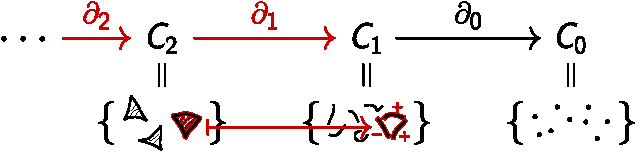
\includegraphics{singular_chaincomplex3}
	\caption{The boundary of a 2-simplex}
	\label{fig:singular_chaincomplex3}
\end{figure}

\todo{Ch: Proposition: $C(X) \in \Ch{\cat{Ab}}$}

\todo{Ch: Example homology of some space}

\todo{Ch: Show that $\Ch{\Ab}$ is an ab. cat. At least show functoriality $\Hom{\Ch{\Ab}}{-}{-}$}


\newpage
\section{Simplicial Abelian Groups}
\label{sec:Simplicial Abelian Groups}

Before defining \emph{simplicial abelian groups}, we will first discuss the more general notion of \emph{simplicial sets}. There are generally two definitions of simplicial sets, an abstract one and a very explicit one. We will start with the abstract one, luckily it can still be visualised in pictures, then we will derive the explicit definition. The reader who is interested in how these notions are developed, should consider reading the introduction by Friedman \cite{friedman}, which also gives nice illustrations.

\subsection{Abstract definition}
\begin{definition}
	We define a category $\DELTA$, where the objects are the finite ordinals $[n] = \{0 < \dots < n\}$ for $n \in \N$ and maps are monotone functions: $\Hom{\DELTA}{[n]}{[m]} = \{ f : [n] \to [m] \I f(i) \leq f(j) \text{ for all } i < j \}$.
\end{definition}

The category $\DELTA$ is sometimes referred to as the \emph{category of finite ordinals} or the \emph{cosimplicial index category}. There are two special kinds of maps in $\DELTA$, the so called \emph{face} maps and \emph{degeneracy} maps. The \emph{$i$-th face maps} $\delta_i: [n-1] \to [n]$ is the unique injective monotone function which \emph{omits} $i$. More precisely, it is defined for all $n \in \Np$ as (note that we do not explicitly denote $n$ in this notation)
$$ \delta_i: [n-1] \to [n], k \mapsto \begin{cases} k & \text{if } k < i,\\ k+1 & \text{if } k \geq i, \end{cases} \hspace{1.0cm} 0 \leq i \leq n. $$

The \emph{$i$-th degeneracy map} $\sigma_i: [n+1] \to [n]$ is the unique surjective monotone function which \emph{hits $i$ twice}. More precisely it is defined for all $n \in \N$ as
$$ \sigma_i: [n+1] \to [n], k \mapsto \begin{cases} k & \text{if } k \leq i,\\ k-1 & \text{if } k > i, \end{cases} \hspace{1.0cm} 0 \leq i \leq n. $$

The nice things about these maps is that every map in $\DELTA$ can be decomposed to a composition of such maps. So in a sense, these are all the maps we need to consider.

\begin{lemma}\emph{(Epi-mono factorization)}
	\label{le:epimono}
	Let $\eta : [m] \to [n]$ be a map in $\DELTA$. Then $\eta$ can be uniquely decomposed as
	$$ \eta = \delta_{i_a} \cdots \delta_{i_1} \sigma_{j_b} \cdots \sigma_{j_1}, $$
	such that $0 \leq j_b < \cdots < j_1 < m$ and $0 \leq i_1 < \cdots < i_a \leq n$.
\end{lemma}
This is called the \emph{epi-mono factorization}, because it factors any map $\eta$ into a surjective part ($\sigma_{j_b} \cdots \sigma_{j_1}$) and an injective part ($\delta_{i_a} \cdots \delta_{i_1}$). In a diagram:

{\centering\begin{tikzpicture}
	\matrix (m) [row sep=1em, column sep=3em, matrix of math nodes]{
		% Note: [] have a meaning in tikz, so I wrapped them in \left \right
		\left[m\right] &     & \left[n\right] \\
		    & \left[k\right] &     \\
	};
	\path[->] (m-1-1) edge node[auto] {$ \eta $} (m-1-3);
	\path[->>] (m-1-1) edge node[below left] {$ \sigma_{j_b} \cdots \sigma_{j_1} $} (m-2-2);
	\path[right hook->] (m-2-2) edge node[below right] {$ \delta_{i_a} \cdots \delta_{i_1} $} (m-1-3);
\end{tikzpicture}\par}

\begin{proof}
	We start with the existence. Consider the set $S = \{ k \in [m-1] \I \eta(k) = \eta(k+1) \}$. These are precisely the elements which are hit twice, now let $S = \{ j_1, \ldots, j_{|S|} \}$ with $0 \leq j_{|S|} < \cdots < j_1 < m$. This gives rise to a surjection $\sigma = \sigma_{j_b} \cdots \sigma_{j_1}: [m] \epi [m-|S|]$.

	Similarly consider $T = \{ k \in [m - |S|] \I k \not \in \eta[m] \}$. These are precisely the elements which are omitted, now let $T = \{ i_1, \ldots, i_{|T|} \}$ with $0 \leq i_1 < \cdots < i_{|T|} \leq n$. This gives an injection $\delta = \delta_{i_a} \cdots \delta_{i_1} : [m - |S|] \mono [n]$. Now we see that $\eta = \delta\sigma$.

	Now for uniqueness, suppose also $\eta = \delta_{i'_{a'}} \cdots \delta_{i'_1} \sigma_{j'_{b'}} \cdots \sigma_{j'_1}$ such that $0 \leq j'_{b'} < \cdots < j'_1 < m$ and $0 \leq i'_1 < \cdots < i'_{a'} \leq n$. It is immediately clear that $b = b'$ must hold by counting the elements which are hit twice, and therefore also $a = a'$. Note that $\eta(j'_k) = \eta(j'_{k+1})$, because the sequences are ordered in the same way, this means $j_k = j'_k$ for all $k$. Similarly $i_k$ = $i'_k$ for all $k$.
\end{proof}

We can now depict the category $\DELTA$ as in Figure~\ref{fig:delta_cat}. Note that the face and degeneracy maps are not unrelated. We will make the exact relations precise later.

\begin{figure}[h!]
	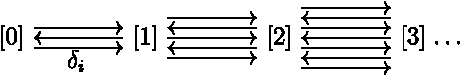
\includegraphics{delta_cat}
	\caption{The category $\DELTA$ with face and degeneracy maps.}
	\label{fig:delta_cat}
\end{figure}

Although this is a very abstract definition, a more geometric intuition can be given. In $\DELTA$ we can regard $[n]$ as an abstract version of the $n$-simplex $\Delta^n$. The face maps $\delta_i$ are then exactly maps which point out how we can embed $[n-1]$ in $[n]$. This is visualized in Figure~\ref{fig:delta_cat_geom}. This picture shows the images of the face maps, for example the image of $\delta_3$ from $[2]$ to $[3]$ is the set $\{0,1,2\}$, which corresponds to the bottom face of the tetrahedron. The degeneracy maps are harder to visualize, one can think of them as ``collapsing'' maps, where two points are identified with each other. For example, this collapses a triangle into a line.

\begin{figure}
	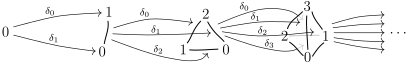
\includegraphics{delta_cat_geom}
	\caption{The category $\DELTA$ with the face maps shown in a geometric way.}
	\label{fig:delta_cat_geom}
\end{figure}

This category $\DELTA$ will act as a prototype for these kind of geometric structures in other categories. This leads to the following definition.

\begin{definition}
	A \emph{simplicial set} $X$ is a functor
	$$X: \DELTA^{op} \to \Set.$$
	(Or equivalently a contravariant functor $X: \DELTA \to \Set.$)
\end{definition}

The category $\sSet$ of all simplicial sets is the functor category $\Set^{\DELTA^{op}}$, where morphisms are natural transformations. Because the face and degeneracy maps give all the maps in $\DELTA$ it is sufficient to define images of $\delta_i$ and $\sigma_i$ in order to define a functor $X: \DELTA^{op} \to \Set$, keeping in mind that these should satisfy some relations which we will discuss next. Hence we can picture a simplicial set as done in Figure~\ref{fig:simplicial_set}. Comparing this to Figure~\ref{fig:delta_cat} we see that the arrows are reversed, because $X$ is a contravariant functor.

\begin{figure}
	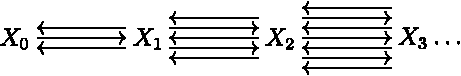
\includegraphics{simplicial_set}
	\caption{A simplicial set.}
	\label{fig:simplicial_set}
\end{figure}


\subsection{Explicit definition}
Of course the maps $\delta_i$ and $\sigma_i$ in $\DELTA$ satisfy certain relations, these are the so called \emph{cosimplicial identities}.

\begin{lemma}
	The face and degeneracy maps in $\DELTA$ satisfy the cosimplicial identities
	\begin{align}
		\delta_j\delta_i &= \delta_i\delta_{j-1},  \hspace{1.5cm} \textnormal{ if } i < j,\\
		\sigma_j\delta_i &= \delta_i\sigma_{j-1},  \hspace{1.5cm} \textnormal{ if } i < j,\\
		\sigma_j\delta_j &= \sigma_j\delta_{j+1} = \id,\\
		\sigma_j\delta_i &= \delta_{i-1}\sigma_j,  \hspace{1.5cm} \textnormal{ if } i > j+1,\\
		\sigma_j\sigma_i &= \sigma_i\sigma_{j+1},  \hspace{1.5cm} \textnormal{ if } i \leq j.
	\end{align}
\end{lemma}
\begin{proof}
	This follows immediately from the definitions.
\end{proof}

Note that these cosimplicial identities are ``purely categorical'', i.e. they only use compositions and identity maps. Because a simplicial set $X$ is a contravariant functor, dual versions of these equations hold in its image. For example, the first equation corresponds to $X(\delta_i)X(\delta_j) = X(\delta_{j-1})X(\delta_i)$ for $i < j$. This can be used for an explicit definition of simplicial sets. In this definition a simplicial set $X$ consists of a collection of sets $X_n$ together with face and degeneracy maps. More precisely:

\begin{lemma}
	A simplicial set $X$ is equivalently specified by a collection sets $X_n$, $n \in \N$, together with functions $d_i: X_n \to X_{n-1}$ and $s_i: X_n \to X_{n+1}$ for $0 \leq i \leq n$ and $n \in \N$, such that the simplicial identities hold
	\begin{align}
		d_i d_j &= d_{j-1} d_i,  \hspace{1.5cm} \text{ if } i < j,\\
		d_i s_j &= s_{j-1} d_i,  \hspace{1.5cm} \text{ if } i < j,\\
		d_j s_j &= d_{j+1} s_j = \id,\\
		d_i s_j &= s_j d_{i-1},  \hspace{1.5cm} \text{ if } i > j+1,\\
		s_i s_j &= s_{j+1} s_i,  \hspace{1.5cm} \text{ if } i \leq j.
	\end{align}
\end{lemma}

It is already indicated that a functor from $\DELTA^{op}$ to $\Set$ is determined when the images for the face and degeneracy maps in $\DELTA$ are provided. So this gives a way of restoring the definition from this specification. Conversely, we can apply functoriality to obtain this specification from the definition. We will not give the proof in more detail. From now on we will use the following notation for a simplicial set $X$:
$$ X_n = X([n]), \quad s_i = X(\sigma_i) \quad\text{and}\quad d_i = X(\delta_i). $$
For any other map $\beta : [n] \to [p]$ we will denote the induced map by $\beta^\ast: X_p \to X_n$.

When using a simplicial set to construct another object, it is often handy to use this second definition, as it gives you a very concrete objects to work with. On the other hand, constructing this might be hard (as you would need to provide a lot of details), in this case we will often use the more abstract definition.

Note that because of the third equation, the degeneracy maps $s_i$ are injective. This means that in the set $X_{n+1}$ there are always ``copies'' of elements of $X_n$. In a way these elements are not interesting, hence we call them degenerate.
\begin{definition}
	An element $x \in X_{n+1}$ is \emph{degenerate} if it lies in the image of $s_i: X_n \to X_{n+1}$ for some $i$, otherwise it is called \emph{non-degenerate}.
\end{definition}
\begin{lemma}
	\label{le:non-degenerate}
	We can write any $x \in X_n$ uniquely as $x = \beta^\ast y$ with $\beta: [n] \epi [m]$ a surjective map and $y \in X_m$ non-degenerate.
\end{lemma}
\begin{proof}
	We will proof the existence by induction over $n$. For $n=0$ the statement is trivial, since all elements in $X_0$ are non-degenerate. Assume the statement is proven for $n$. Let $x \in X_{n+1}$. Clearly if $x$ itself is non-degenerate, we can write $x = \id^\ast x$. Otherwise it is of the form $x = s_i x'$ for some $x' \in X_n$ and $i$. The induction hypothesis tells us that we can write $x' = \beta^\ast y$ for some surjection $\beta: [n] \epi [m]$ and $y \in X_m$ non-degenerate. So $x = s_i \beta^\ast y = (\beta \sigma_i)^\ast y$.

	For uniqueness, assume $x = \beta^\ast y = \gamma^\ast z$ with $\beta: [n] \epi [m]$, $\gamma: [n] \epi [m']$ and $y \in X_m, z \in X_{m'}$ non-degenerate. Because $\beta$ is surjective there is an $\alpha:[m]\to[n]$ such that $\beta\alpha = \id$ and hence $y = \alpha^\ast \gamma^\ast z = (\gamma\alpha)^\ast z$. By the epi-mon factorization (Lemma~\ref{le:epimono}) we can write $\gamma\alpha = \delta_{i_a} \cdots \delta_{i_1} \sigma_{j_b} \cdots \sigma_{j_1}$, using that $y$ is non-degenerate we know that $\gamma\alpha$ is injective. So we have $\gamma\alpha: [m] \mono [m']$. Because of symmetry (of $y$ and $z$) we also have some map $[m'] \mono[m]$, so $m = m'$. So $\gamma\alpha$ is also surjective, hence the identity function, thus $y = z$, meaning that the non-degenerate $m$-simplex is unique.

	Now assume $x = \beta^\ast y = \gamma^\ast y$ with $\gamma, \beta: [n] \epi [m]$ such that $\beta \neq \gamma$, and $y \in X_m$ non-degenerate. Then we can find an $\alpha:[m]\to[n]$ such that $\beta\alpha = \id$ and $\gamma\alpha \neq \id$. With the epi-mono factorization write $\gamma\alpha = \delta_{i_a} \cdots \delta_{i_1} \sigma_{j_b} \cdots \sigma_{j_1}$, then by functoriality of $X$
	$$ y = \alpha^\ast \beta^\ast y = \alpha^\ast \gamma^\ast y = s_{j_1} \cdots s_{j_b} d_{i_1} \cdots d_{i_a} y. $$
	Note that $y$ was non-degenerate, so $s_{j_1} \cdots s_{j_b} = \id$, hence $d_{i_1} \cdots d_{i_a} = \id$. So $\gamma\alpha = \id$, which gives a contradiction. So $\beta = \gamma$, meaning that the surjection $\beta$ is also unique.
\end{proof}

\subsection{The standard $n$-simplex}
Recall that for any category $\cat{C}$ we have the $\mathbf{Hom}$-functor $\Hom{\cat{C}}{-}{-}: \cat{C}^{op} \times \cat{C} \to \Set$. We can fix an object $C \in \cat{C}$ and get a functor $\Hom{\cat{C}}{-}{C} : \cat{C}^{op} \to \Set$. In our case we can get the following simplicial sets in this way:

\begin{definition}
	The \emph{standard $n$-simplex} $\Delta[n] \in \sSet$ is given by
	$$\Delta[n] = \Hom{\DELTA}{-}{[n]} : \DELTA^{op} \to \Set.$$
\end{definition}

Note that $\Delta[-]: \DELTA \to \sSet$ is exactly the Yoneda embedding. In a moment we will see why the Yoneda lemma is useful to us, but let us first explicitly describe two examples of such standard simplices.

\begin{example}
	We will compute how $\Delta[0]$ look like. Note that $[0]$ is an one-element set, so for any set $S$, there is only one function $\ast: S \to [0]$. Hence $\Delta[0]_n = \{\ast\}$ for all $n$ and the face and degeneracy maps are necessarily the identity maps $\id: \{\ast\} \to \{\ast\}$. Thus, $\Delta[0]$ looks like
	$$ \Delta[0] :=
	\begin{tikzpicture}[baseline=-0.5ex]
	\matrix (m) [matrix of math nodes] { 
		\{\ast\} & \{\ast\} & \{\ast\} & \cdots \\
	}; 

	\foreach \r in {-5, 5} \draw [raise line=\r, <-] (m-1-1) -> (m-1-2);
	\foreach \r in {0} \draw [raise line=\r, ->] (m-1-1) -> (m-1-2);

	\foreach \r in {-10, 0, 10} \draw [raise line=\r, <-] (m-1-2) -> (m-1-3);
	\foreach \r in {-5, 5} \draw [raise line=\r, ->] (m-1-2) -> (m-1-3);

	\foreach \r in {-15, -5, 5, 15} \draw [raise line=\r, <-] (m-1-3) -> (m-1-4);
	\foreach \r in {-10, 0, 10} \draw [raise line=\r, ->] (m-1-3) -> (m-1-4);
	\end{tikzpicture}.$$
	Note that the only non-degenerate simplex is the unique $0$-simplex.
\end{example}

\begin{example}
	$\Delta[1]$ is a bit more interesting, but still not too complicated. We will describe the first three sets $\Delta[1]_0$, $\Delta[1]_1$ and $\Delta[1]_2$. We can use the fact that any monotone function $f: [n] \to [m]$ is a composition of first applying degeneracy maps, and then face maps, i.e.: $f: [n] \tot{\sigma_{i_0} \cdots \sigma_{i_M}} [k] \tot{\delta_{j_0} \cdots \delta_{j_N}} [m]$, where $k \leq m, n$.

	For $\Delta[1]_0$ we have to consider maps from $[0]$ to $[1]$, we cannot first apply degeneracy maps (there is no object $[-1]$). So this leaves us with the face maps: $\Delta[1]_0 = \{\delta_0, \delta_1\}$. For $\Delta[1]_1$ we of course have the identity function and two functions $\delta_0\sigma_0, \delta_1\sigma_0$. Now $\Delta[1]_2$ are the maps from $[2]$ to $[1]$.

	We will compute the two face maps $d_0$ and $d_1$ from $\Delta[1]_1$ to $\Delta[1]_0$. Recall that the $\mathbf{Hom}$-functor in the first argument (the contravariant argument) works with precomposition. So this gives
	\begin{align*}
		d_0(\id) &= \id \delta_0 = \delta_0 \\
		d_0(\delta_0\sigma_0) &= \delta_0 \sigma_0 \delta_0 = \delta_0 \\
		d_0(\delta_1\sigma_0) &= \delta_0 \sigma_0 \delta_0 = \delta_1.
	\end{align*}
	Where we in the first calculation used the identity law. In the second and third line we used the third simplicial equation, asserting that $\sigma_0 \delta_0 = \id$. Similarly we can calculate the face map $d_1$:
	\begin{align*}
		d_1(\id) &= \id \delta_1 = \delta_1 \\
		d_1(\delta_0\sigma_0) &= \delta_0 \sigma_0 \delta_1 = \delta_0 \\
		d_1(\delta_1\sigma_0) &= \delta_0 \sigma_0 \delta_1 = \delta_1.
	\end{align*}

	$$ \Delta[1] :=
	\begin{tikzpicture}[baseline=-0.5ex]
	\matrix (m) [matrix of math nodes] { 
		\{\delta_0, \delta_1\} & \{\delta_0 \sigma_0, \id, \delta_1 \sigma_0\} & \cdots \\
	}; 

	\foreach \r in {-5, 5} \draw [raise line=\r, <-] (m-1-1) -> (m-1-2);
	\foreach \r in {0} \draw [raise line=\r, ->] (m-1-1) -> (m-1-2);

	\foreach \r in {-10, 0, 10} \draw [raise line=\r, <-] (m-1-2) -> (m-1-3);
	\foreach \r in {-5, 5} \draw [raise line=\r, ->] (m-1-2) -> (m-1-3);

	\end{tikzpicture}.$$
	In this simplicial set there are three non-degenerate simplices. There is $\id \in \Delta[1]_1$, which clearly is non-degenerate, and the two $0$-simplices $\delta_0$ and $\delta_1$. One can think of this simplicial set as a line (the non-degenerate $1$-simplex) with its endpoints (the two $0$-simplices).
\end{example}

\subsection{Simplicial objects in arbitrary categories}
Of course the definition of simplicial set can easily be generalized to other categories. For any category $\cat{C}$ we can consider the functor category $\cat{sC} = \cat{C}^{\DELTA^{op}}$. In this thesis we are interested in the category of \emph{simplicial abelian groups}:
$$ \sAb = \Ab^{\DELTA^{op}}. $$
So a simplicial abelian group $A$ is a collection of abelian groups $A_n$, together with face and degeneracy maps, which in this case means group homomorphisms $d_i$ and $s_i$ such that the simplicial equations hold.

Note that the set of natural transformations between two simplicial abelian groups $A$ and $B$ is also an abelian group. The proof that $\sAb$ is a preadditive category is very similar to the proof we saw in Section~\ref{sec:Chain Complexes}. For two natural transformations $f,g: A \to B$ we simply define $f+g$ pointwise by $(f+g)_n = f_n + g_n$ and it is easily checked that this is a natural transformation.

As we are interested in simplicial abelian groups, it would be nice to obtain simplicial abelian groups associated to the standard $n$-simplices. We have seen how to make an abelian group out of any set using the free abelian group functor. We can use this functor $\Z[-]: \Set \to \Ab$ to induce a functor $\Z^\ast[-]: \sSet \to \sAb$ as shown in the following diagram.
\begin{figure}[h!]
	\begin{tikzpicture}
		\matrix (m) [matrix of math nodes]{
			\DELTA^{op} & \Set \\
			            & \Ab  \\
		};
		\path[->]
		(m-1-1) edge node[auto] {$ X $} (m-1-2)
		(m-1-2) edge node[auto] {$ \Z[-] $} (m-2-2)
		(m-1-1) edge node[below left] {$ \Z^\ast[X] $} (m-2-2);
	\end{tikzpicture}
	\caption{The simplicial set $X$ can be made into a simplicial abelian group $\Z^\ast[X]$ by postcomposing with $\Z[-]$.}
	\label{fig:diagram_Z}
\end{figure}
This construction obviously defines a functor $\Z^\ast[-] : \sSet \to \sAb$. Similarly, postcomposition with the forgetful functor $U: \Ab \to \Set$ gives rise to a forgetful functor $U^\ast: \sAb \to \sSet$. Thus in formulas we have
$$ \Z^\ast[X]_n = \Z[X_n] \quad\text{and}\quad U^\ast(A)_n = U(A_n). $$
This justifies that we may drop this extra decoration ($^\ast$) and write $\Z[-]$ (resp. $U$) instead of $\Z^\ast[-]$ (resp. $U^\ast$).

\begin{lemma}
	The functor $\Z[-]: \sSet \to \sAb$ is a left adjoint, with $U: \sAb \to \sSet$ as right adjoint.
\end{lemma}
\begin{proof}
	First we note that $U\Z[X]_n = U\Z[X_n]$ by definition, so pointwise we get (by the fact that $\Z$ and $U$ already form an adjunction):
\begin{center}
	\begin{tikzpicture}
		\matrix (m) [matrix of math nodes]{
			X_n & U\Z[X]_n & \Z[X_n] \\
			    & U(A_n)   & A_n \\
		};
		\path[->]
		(m-1-1) edge node[auto] {$ i $} (m-1-2)
		(m-1-2) edge node[auto] {$ U(\overline{f}) $} (m-2-2)
		(m-1-1) edge node[auto] {$ f $} (m-2-2);
		\path[->]
		(m-1-3) edge node[auto] {$ \overline{f} $} (m-2-3);
	\end{tikzpicture}
\end{center}
	Then use naturality of $i$ (in $X_n$, thus in particular in $n$) to extend this to $i^\ast : X \to U\Z[X]$. Now if we are given a natural transformation $f: X \to UA$ of simplicial sets we can again construct $\overline{f}: \Z[X] \to A$ pointwise. The reader is invited to check the details.
\end{proof}

\begin{example}
	We can apply this to the standard $n$-simplex $\Delta[1]$. This gives $\Delta[1]_0 \iso \Z^2$, since $\Delta[1]_0$ has two elements, and $\Z^\ast[\Delta[1]]_1 \iso \Z^3$, where the isomorphisms are taken such that
	\begin{align*}
		\delta_0         &\mapstot{\iso} (1, 0), \\
		\delta_1         &\mapstot{\iso} (0, 1), \\
		\delta_0\sigma_0 &\mapstot{\iso} (1, 0, 0), \\
		\id              &\mapstot{\iso} (0, 1, 0), \\
		\delta_1\sigma_0 &\mapstot{\iso} (0, 0, 1).
	\end{align*}
	The face maps from $\Z[\Delta[1]]_1$ to $\Z[\Delta[1]]_0$ under these isomorphisms are then given by
	\begin{align*}
		d_0(x, y, z) &= (x+y, z), \\
		d_1(x, y, z) &= (x, y+z).
	\end{align*}
\end{example}

\subsection{The Yoneda lemma}
Recall the statement of the Yoneda lemma from Section~\ref{sec:Category Theory}. In our case we consider functors $X: \DELTA^{op} \to \Set$ and objects $[n]$. So this gives us a natural bijection
$$ \Hom{\sSet}{\Delta[n]}{X} \iso X_n $$
telling us that we can regard $n$-simplices in $X$ as maps from $\Delta[n]$ to $X$. This also extends to the case of simplicial abelian groups.
\begin{lemma}\emph{(The additive Yoneda lemma)}
	Let $A$ be a simplicial abelian group. Then there is a group isomorphism
	$$ \Hom{\sAb}{\Z[\Delta[n]]}{A} \iso A_n, $$
	which is natural in $A$ and $[n]$.
\end{lemma}
\begin{proof}
	By using the (non-additive) Yoneda lemma and the fact that $\Z$ is a left adjoint, we already have a natural bijection:
	$$ \Hom{\sAb}{\Z[\Delta[n]]}{A} \iso \Hom{\sSet}{\Delta[n]}{U(A)} \iso U(A)_n = A_n. $$
	The only thing that we need to check is that this bijection preserves the group structure. Recall that this bijection from $\Hom{\sAb}{\Z[\Delta[n]]}{A}$ to $A_n$ is given by (where $\id = \id_{[n]}$ is a generator in $\Z[\Delta[n]]$)
	$$ \phi(f) = f_n(\id) \in X_n \quad\text{ for } f: \Delta[n] \to X. $$

	Now let $A$ be a simplicial abelian group and $f, g: \Z\Delta[n] \to A$ maps. Then we compute
	$$ \phi(f) + \phi(g) = f_n(\id) + g_n(\id) = (f_n + g_n)(\id) = (f+g)_n(\id) = \phi(f+g), $$
	where we regard $\id \in \Delta[n]$ as an element $\id \in \Z\Delta[n]$, we can do so by the unit of the adjunction. So this bijection is also a group homomorphism, hence we have an isomorphism $\Hom{\sAb}{\Z[\Delta[n]]}{A} \iso A_n$ of abelian groups.
\end{proof}


\newpage
\section{Constructions}
\label{sec:Constructions}

Comparing chain complexes and simplicial abelian groups, we see a similar structure. Both objects consists of a sequence of abelian groups, with maps in between. At first sight simplicial abelian groups have more structure, because there are maps in both directions. It is not clear how to make degeneracy maps given a chain complex, in fact it is already unclear how to define more maps (the face maps) out of one (the boundary one). Constructing a chain complex from a simplicial abelian group on the other hand seems doable.

\subsection{Unnormalized chain complex}
Given a simplicial abelian group $A$, we have a family of abelian groups $A_n$. We define a grouphomomorphism $\del_{n-1} : A_n \to A_{n-1}$ as:
$$\del_{n-1} = d_0 - d_1 + \ldots + (-1)^n d_n \text{ for every } n > 0.$$
\begin{lemma}
	Using $A_n$ as the family of abelian groups and the maps $\del_n$ as boundary maps gives a chain complex.
\end{lemma}
\begin{proof}
	We already have a collection of abelian groups together with maps, so the only thing to proof is $\del_n \circ \del_{n+1} = 0$.

	\todo{C: insert calculation with sums}

	So indeed this is a chain complex.
\end{proof}

This construction gives a functor $C : \sAb \to \Ch{\Ab}$\todo{C: prove this? Is it a adjunction?}. And in fact we already used it in the construction of the singular chaincomplex, where we defined the boundary maps as $\del(\sigma) = \sigma \circ d_0 - \sigma \circ d_1 + \ldots + (-1)^{n+1} \sigma \circ d_{n+1}$ (on generators). The terms $\sigma \circ d_i$ are the maps given by the $\mathbf{Hom}$-functor from $\Top$ to $\Set$, in fact this $\mathbf{Hom}$-functor can be used to get a functor $Sing : \Top \to \sSet$, applying the free abelain group pointwise give a functor $\Z^\ast : \sSet \to \sAb$, and finally using the functor $C$ gives the singular chain complex.
\todo{C: is this a nice thing to add?}

Let us investigate whether this functor can be used for our sought equivalence. For a functor from $\Ch{\Ab}$ to $\sAb$ we cannot simply take the same collection of abelian groups. This is due to the fact that the degenracy maps should be injective. This means that for a simplicial abelian group $A$, if we know $A_n$ is non-trivial, then all $A_m$ for $m > n$ are also non-trivial.

But for chain complexes it \emph{is} possible to have trivial abelian groups $C_m$, while there is a $n < m$ with $C_n$ non-trivial. Take for example the chain complex $ C = \ldots \to 0 \to 0 \to \Z $. Now if we would construct a (non-trivial) simplicial abelian group $K(C)$ from this chain complex, we now know that $K(C)_n$ is non-trivial for all $n \in \N$. This means that $C(K(C))_n$ is non-trivial for all $n \in \N$. For an equivalence we require a (natural) isomorphism: $C(K(C)) \tot{\iso} C$, this in particular means an isomorphism in each degree $n > 0$: $ 0 \neq C(K(C))_n \tot{\iso} C_n = 0 $, which is not possible. So the functor $C$, as defined as above, will not give us the equivalence we wanted, although it is a very nice functor.

\subsection{Normalized chain complex}
To repair this defect we should be more careful. Given a simplicial abelian group, simply taking the same collection for our chain complex will not work (as shown above). Instead we are after some ``smaller'' abelian groups, and in some cases the abelian groups should completely vanish (as in the example above).

Given a simplicial abelian group $A$, we define abelian groups $N(A)_n$ as:
$$ N(A)_n = \bigcap_{i=1}^{n} \ker(d_i : A_n \to A_{n-1}). $$
Now define grouphomomorphisms $\del : N(A)_n \to N(A)_{n-1}$ as:
$$ \del = d_0|_{N(A)_n}. $$
\begin{lemma}
	The function $ \del $ is well-defined. Furthermore $ \del \circ \del = 0 $, hence $N(A)$ is a chain complex.
\end{lemma}
\begin{proof}
	\todo{C: This is easy}
\end{proof}

\todo{C: As an example calculate $N(\Z[\Delta[0]])$}


\subsection{From $\Ch{\Ab}$ to $\sAb$}
For the other way around we actually get a functor for free, via abstract nonsense. Let $F : \sAb \to A$ be any functor, where $A$ is an abelian category. We are after a functor $G : A \to \sAb$, this means that if we are given $C \in A$, we are looking for a functor $G(C) : \DELTA^{op} \to \Ab$. Fixing $C$ in the second argument of the $\mathbf{Hom}$-functor gives: $\Hom{A}{-}{C} : A^{op} \to \Ab$, because $A$ is an abelian category. We see that the codomain of this functor already looks good, now if we have some functor from $\DELTA^{op}$ to $A^{op}$, we can precompose, to obtain a functor from $\DELTA^{op}$ to $\Ab$.

Now recall that we have a family of protoype simplicial sets $\Delta[n]$, which are given by the functor $\Delta : \DELTA \to \sSet$. We can apply the free abelian group pointwise, which gives a functor $\Z^{\ast} : \sSet \to \sAb$. And finally we have our functor $F : \sAb \to A$. Composing these gives:
$$ F \Z^{\ast} \Delta : \DELTA \to A. $$
We can formally regard this functor as a functor from $\DELTA^{op}$ to $A^{op}$. Now combining this with the $\mathbf{Hom}$-functor gives:
$$ \Hom{A}{F \Z^{\ast} \Delta (-)}{C} : \DELTA^{op} \to \Ab. $$
Now this is a functor, because it is a composition of functors. Furthermore it is also functorial in the second argument, giving a functor
$$ \Hom{A}{F \Z^{\ast} \Delta (-)}{-} : A \to \sAb $$
where we are supposed to fill in the second argument first, leaving us with a simplicial abelian group.

Now we know that $\Ch{\Ab}$ is an abelian group and we have actually two functors $C, N : \sAb \to \Ch{\Ab}$, so we now have functors from $\Ch{\Ab} \to \sAb$. Of course we will be interested in the one using $N$. So we define the functor:
$$ K(C) = \Hom{\Ch{\Ab}}{N\Z^\ast\Delta[-]}{C} \in \sAb. $$
This definitions is very abstract, but luckily we can also give a more explicit definition. By writing it out for low dimensions we see:

$$ K(C)_0 = \Hom{\Ch{\Ab}}{N\Z^\ast\Delta[0]}{C} = \Bigg\{
\begin{tikzpicture}[baseline=-0.5ex]
	\matrix (m) [matrix of math nodes, row sep=1em, column sep=1em] { 
		\cdots  & 0 & 0 & \Z  \\
		\cdots  & C_2 & C_1 & C_0 \\
	}; 

	\foreach \x in {1, 2}
		\foreach \i/\j in {1/2, 2/3, 3/4} \draw[->] (m-\x-\i) -- (m-\x-\j);
	
	\foreach \i/\j in {2/2, 3/1, 4/0} \draw[->] (m-1-\i) -- node {$f_\j$} (m-2-\i);
\end{tikzpicture}
\Bigg\} \iso C_0, $$
because for $f_1, f_2, \ldots$ there is now choice at all, and for $f_0 : \Z \to C_0$ we only have to choose an image for $1 \in \Z$. In the next dimension we see:

$$ K(C)_1 = \Hom{\Ch{\Ab}}{N\Z^\ast\Delta[1]}{C} = \Bigg\{
\begin{tikzpicture}[baseline=-0.5ex]
	\matrix (m) [matrix of math nodes, row sep=1em, column sep=1em] { 
		\cdots  & 0 & \Z & \Z^2  \\
		\cdots  & C_2 & C_1 & C_0 \\
	}; 

	\foreach \x in {1, 2}
		\foreach \i/\j in {1/2, 2/3, 3/4} \draw[->] (m-\x-\i) -- (m-\x-\j);
	
	\foreach \i/\j in {2/2, 3/1, 4/0} \draw[->] (m-1-\i) -- node {$f_\j$} (m-2-\i);
\end{tikzpicture}
\Bigg\} \iso C_1 \oplus C_0, $$

because again we can choose $f_1$ anyway we want, which gives us $C_1$. But then we are forced to choose $f_0(x, x) = \del(f_1(x))$ for all $x \in \Z$, so we are left with choosing an element $c \in C_0$ for defining $f(1,-1) = c$. Adding this gives $C_1 \oplus C_0$. This pattern can be continued and gives the following result:

\begin{proposition}
	For any chain complex $C$ we have $K(C)_n \iso \bigoplus_{[n] \epi [p]} C_p$.
\end{proposition}


\newpage
\section{Homotopy}
\label{sec:Homotopy}

We've already seen homology in chain complexes. We can of course now translate this notion to simplicial abelian groups, by assigning a simplicial abelian group $X$ to $H_n(N(X))$. But there is a more general notion of homotopy for simplicial sets, which is also similar to the notion of homotopy in topology. We will define the notion of homotopy groups for simplicial sets.

When dealing with homotopy in a topological space $X$ we always need a base-point $\ast \in X$. This is also the case for homotopy in simplicial sets. We will notate the chosen base-point of a simplicial set $X$ with $\ast \in X_0$. Note that it is a $0$-simplex, but in fact the base-point is present in all sets $X_n$, because we can consider its degenerate simplices $s_0(\ldots(s_0(\ast))\ldots) \in X_n$, we will also denote these elements as $\ast$. Of course in our situation we are concerned about simplicial abelien groups, where there is an obvious choice for the base-point, namely $0$.

\subsection{Homotopy groups}
\begin{definition}
	Given a simplicial set $X$ with base-point $\ast$, we define $Z_n(X)$ to be the set of $n$-simplices with the base-point as boundary, i.e.:
	$$ Z_n(X) = \{ x \in X_n | d_i(x) = \ast \text{ for all } i \leq n \}. $$
	For two $n$-simplices $x, x' \in Z_n(X)$, we define $x \sim x'$ if there exists $y \in X_{n+1}$ such that:
	\begin{align}
		d_0(y) &= x \\
		d_1(y) &= x' \\
		d_i(y) &= \ast \text{ for all } i > 1.
	\end{align}
	We will call $y$ the \emph{homotopy} and notate $y: x \sim x'$.
\end{definition}

Of course we would like $\sim$ to be an equivalence relation, however this is not true for all simplicial sets. For example there is in general no reason for symmetry, existence of a $1$-simplex $y$ from $x$ to $x'$ does not give us a $1$-simplex $y'$ from $x'$ to $x$. One can give an precise condition on when it is a equivalence relation, the so called \emph{Kan-condition}. In our case of simplicial abelien groups, however, we can prove directly that $\sim$ is an equivalence relation.

In figure~\ref{fig:simplicial_htp} it is shown why the definition of homotopy makes sense for $n=1$. Two homotopic $1$-simplices from $Z_n(X)$ are depicted in two ways. The first way only shows the structure we have, indicating what the boundaries are (as described by the face maps). In the second figure we collapsed all occurences of $0$ into a single point. This way of drawing a homotopy should remind the reader of homotopy (between paths) in a topological space.

\begin{figure}[h!]
\begin{subfigure}{.5\textwidth}
  \centering
  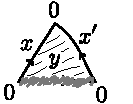
\includegraphics{simplicial_htp1}
\end{subfigure}%
\begin{subfigure}{.5\textwidth}
  \centering
  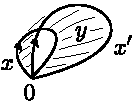
\includegraphics{simplicial_htp2}
\end{subfigure}
\caption{In the figure on the left two homotopic $1$ simplices $x, x' \in Z_n(X)$ are shown. The fact that $d_2(y) = \ast$ is depicted by crossing out the bottom line. The right image shows exactly the same structure if we would draw the $0$-simplex $0$ only once (and hence also collapse the degenerate $1$-simplex $d_2y$).}
\label{fig:simplicial_htp}
\end{figure}

\begin{lemma}
	The relation $\sim$ as defined above is an equivalence relation on $Z_n(X)$. Furthermore it is compatible with addition.
\end{lemma}

Before proving this, one should have a look at figure~\ref{fig:simplicial_eqrel}. In this figure we show what we want to proof in degree $n=0$ (i.e. the simplices of interest are points, and the homotopies are paths).

\begin{figure}[h!]
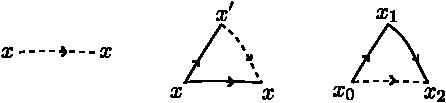
\includegraphics{simplicial_eqrel}
\caption{The three properties of an equivalence relation: reflexivity, symmetry and transitivity. The dashed lines show which homotopy we should construct.}
\label{fig:simplicial_eqrel}
\end{figure}

\begin{proof}
	\emph{Reflexivity}. Let $x \in Z_n(X)$, define $y = s_0 x$. By considering the simplicial identities $d_0 s_0 = \id$ and $d_1 s_0 = \id$, it follows that $d_0 y = d_1 y = x$. Furthermore $d_i y = d_i s_0 x = s_0 d_{i-1} x = 0$ for all $i > 1$, because $x \in Z_n(X)$.

	\emph{Symmetry}. Let $x, x' \in Z_n(X)$ with $y: x \sim x'$. Define $y' = s_0 x + s_0 x' - y$, then by using linearity: $d_0 y' = x + x' - x = x'$ and $d_1 y' = x + x' - x' = x$. For $i>1$ we again get $d_i y' = 0$, because $x \in Z_n(X)$.

	\emph{Transitivity}. Let $x_0, x_1, x_2 \in Z_n(X)$ with $y: x_0 \sim x_1$ and $z: x_1 \sim x_2$. Define $w = y + z - s_0 x_1$. By linearity we have $d_0 w = x_0 + x_1 -x_1 = x_0$, similarly $d_1 w = x_2$. Again for $i>1$ we have $d_i w = 0$.

	\emph{Addition}. Let $y: x_0 \sim x_1$ and $z: x_2 \sim x_3$. Then by linearity $y + g: x_0 + x_2 \sim x_1 + x_3$ and $-y: -x_0 \sim -x_1$.
\end{proof}

\begin{definition}
	Given a simplicial abelian group $X$, we define the $n$-th homotopy group as:
	$$ \pi_n(X) = Z_n(X) / \sim. $$
\end{definition}

Note that this is an abelian group, because $Z_n(X)$ is a subgroup of $X_n$, and $\sim$ also defines a subgroup. It is relatively straight forward to prove that this definition coincides with the $n$-th homology group of the associated normalized chain complex.

\begin{lemma}
	For any simplicial abelian group $X$:
	$$ \pi_n(X) = H_n(N(X)). $$
\end{lemma}
\begin{proof}
	By writing out the definitions of the $n$-cycles and $n$-boundaries of the normalized chain complex, we see:
	\begin{align*}
		\ker(\del) &= \{ x \in N(X)_n \I \del(x) = 0 \} \\
			&= \{ x \in X_n \I d_i(x) = 0 \text{ forall } i > 0 \text{ and } d_0(x) = 0 \} \\
			&= \{ x \in X_n \I d_i(x) = 0 \text{ forall } i \leq n \} \\
			&= Z_n(X) \\
		\im(\del) &= \{ \del(y) \I y \in N(X)_{n+1} \} \\
			&= \{ d_0 y \I y \in X_{n+1}, d_i(y) = 0 \text{ for all } i > 0 \} \\
			&= \{ x \in N(X)_n \I x \sim 0 \}
	\end{align*}
	So we see that $\pi_n(X) = Z_n(X) / \sim = \ker(\del) / \im(\del) = H_n(N(X))$.
\end{proof}

\begin{corollary}
	For a chain complex $C$ we have $H_n(C) \iso \pi_n(K(C))$
\end{corollary}
\begin{proof}
	By the established equivalence we have for any chain complex $C$:
	$$ \pi_n(K(C)) \iso H_n(N(K(C))) \iso H_n(C). $$
\end{proof}

\subsection{Topology}
In section~\ref{sec:Constructions} we saw that we can construct a functor $G: \cat{C} \to \sSet$ if we are provided a functor the other way around. If we can define a functor $F: \DELTA \to \Top$, then for any space $X$ we have a simplicial set $\Hom{\Top}{F-}{X}: \DELTA^{op} \to \Set$. In section~\ref{sec:Chain Complexes}, we already defined the \emph{topological $n$-simplex} $\Delta^n$ and face maps $\delta^i : \Delta^n \mono \Delta^{n+1}$. We can similarly define degeneracy maps $s^i: \Delta^n \to \Delta^{n-1}$ as:
$$ s^i(x_0, \ldots, x_n) = (x_0, \ldots, x_i + x_{i+1}, \ldots, x_n) \in \Delta^{n-1}. $$
The reader is invited to check the cosimplicial identities himself and conclude that we now have a functor $F: \DELTA \to \Top$, and hence we have a functor $S: \Top \to \sSet$ given by:
$$ \text{Sing}(X)_n = \Hom{\Top}{\Delta^n}{X}. $$

Recall construction of the singular chain complex in section~\ref{sec:Chain Complexes}:
$$ C_n(X) = \Z[\Hom{\cat{Top}}{\Delta^n}{X}]. $$
Where the boundary map was given as an alternating sum. Looking more closely we see that this construction decomposes as:
$$ C: \Top \tot{\text{Sing}} \sSet \tot{\Z^\ast} \sAb \tot{C} \Ch{\Ab}, $$
where the last functor is the \emph{unnormalized chain complex}. All the categories involved have a notion of homotopy. In topological spaces this is the known notion where $f, g:X \to Y$ are homotopic if there exists a homotopy $H:I \times X \to Y$ with the appropriate properties. In simplicial sets (or simplicial abelian groups) we only saw the notion of homotopy groups, but there exists a more general notion of homotopy, as discussed in the overview of Friedman \cite{friedman}. And finally in chain complexes we saw homology groups, but this category also has a more general notion of chain homotopy, which can be found in any book on homological algebra such as in the book of Rotman \cite{rotman}.

It is known that for any simplicial abelian group both the normalized and unnormalized chain complex have the same homology groups. More precisely for any simplicial abelian group $X$ we have:
$$ H_n(N(X)) \iso H_n(C(X)) \quad\text{for all } n \in \N. $$
This is for example proven in \cite[Theorem 4.1]{eilenberg}. So this assures that the homology groups of the singular chain complex of a space are really the homotopy groups of the simplicial abelian group which is in the background.


\newpage
\todo{References: Lamotke, Friedman, Weibel}

\newpage
\listoftodos
% \nocite{*}
% \bibliographystyle{alpha}
% \bibliography{references}	
\end{document}
